% Explain the atomic island concept
% Inter atomic-island switches
% Explain how this will be the grid we'll be optimizing on
% Explain that we can merge in the atomic islands acting as "leafs" (show comparison graph)grid
% Explain the problem with not connected parts of the grid in the satandard switch case and the solution

To test out different gird configurations some data preparation is required. The following
steps will be showcased utilizing suburban grid data from the aforementioned
Swiss grid operator. The data has been loaded through API calls specified in
\autoref{sec:appendix:api}.\\ For this example
a grid area with the following elements was chosen:

\begin{figure}[H]
    \begin{center}
        \begin{tabular}{ll}
            Grids & 5\\
            Nodes (all types) & 2890\\
            Edges (all types) & 2958\\
            Transformer & 10\\
            Cables & 1995\\
            Prosumers & 600\\
            Switches & 152\\
        \end{tabular}
    \end{center}
    \caption{
        Number of grid elements in the chosen example grid area within a Swiss suburb.
    }
    \label{table:data_prep:swiss_suburban_numbers}
\end{figure}

\subsection{Atomic islands}

To make topological analysis easy and performant atomic islands will be formed.
Figure \ref{fig:data_prep:atomic_islands}
shows some arbitrary grid topology with some nodes and edges. Atomic islands are clusters
of nodes and edges which can not be subdivided by switches further. In the example shown
it is easy to see that two non-divisible clusters can be formed. One containing nodes
1 to 4 and one containing nodes 5 to 8.

\begin{figure}[H]
    \begin{center}
        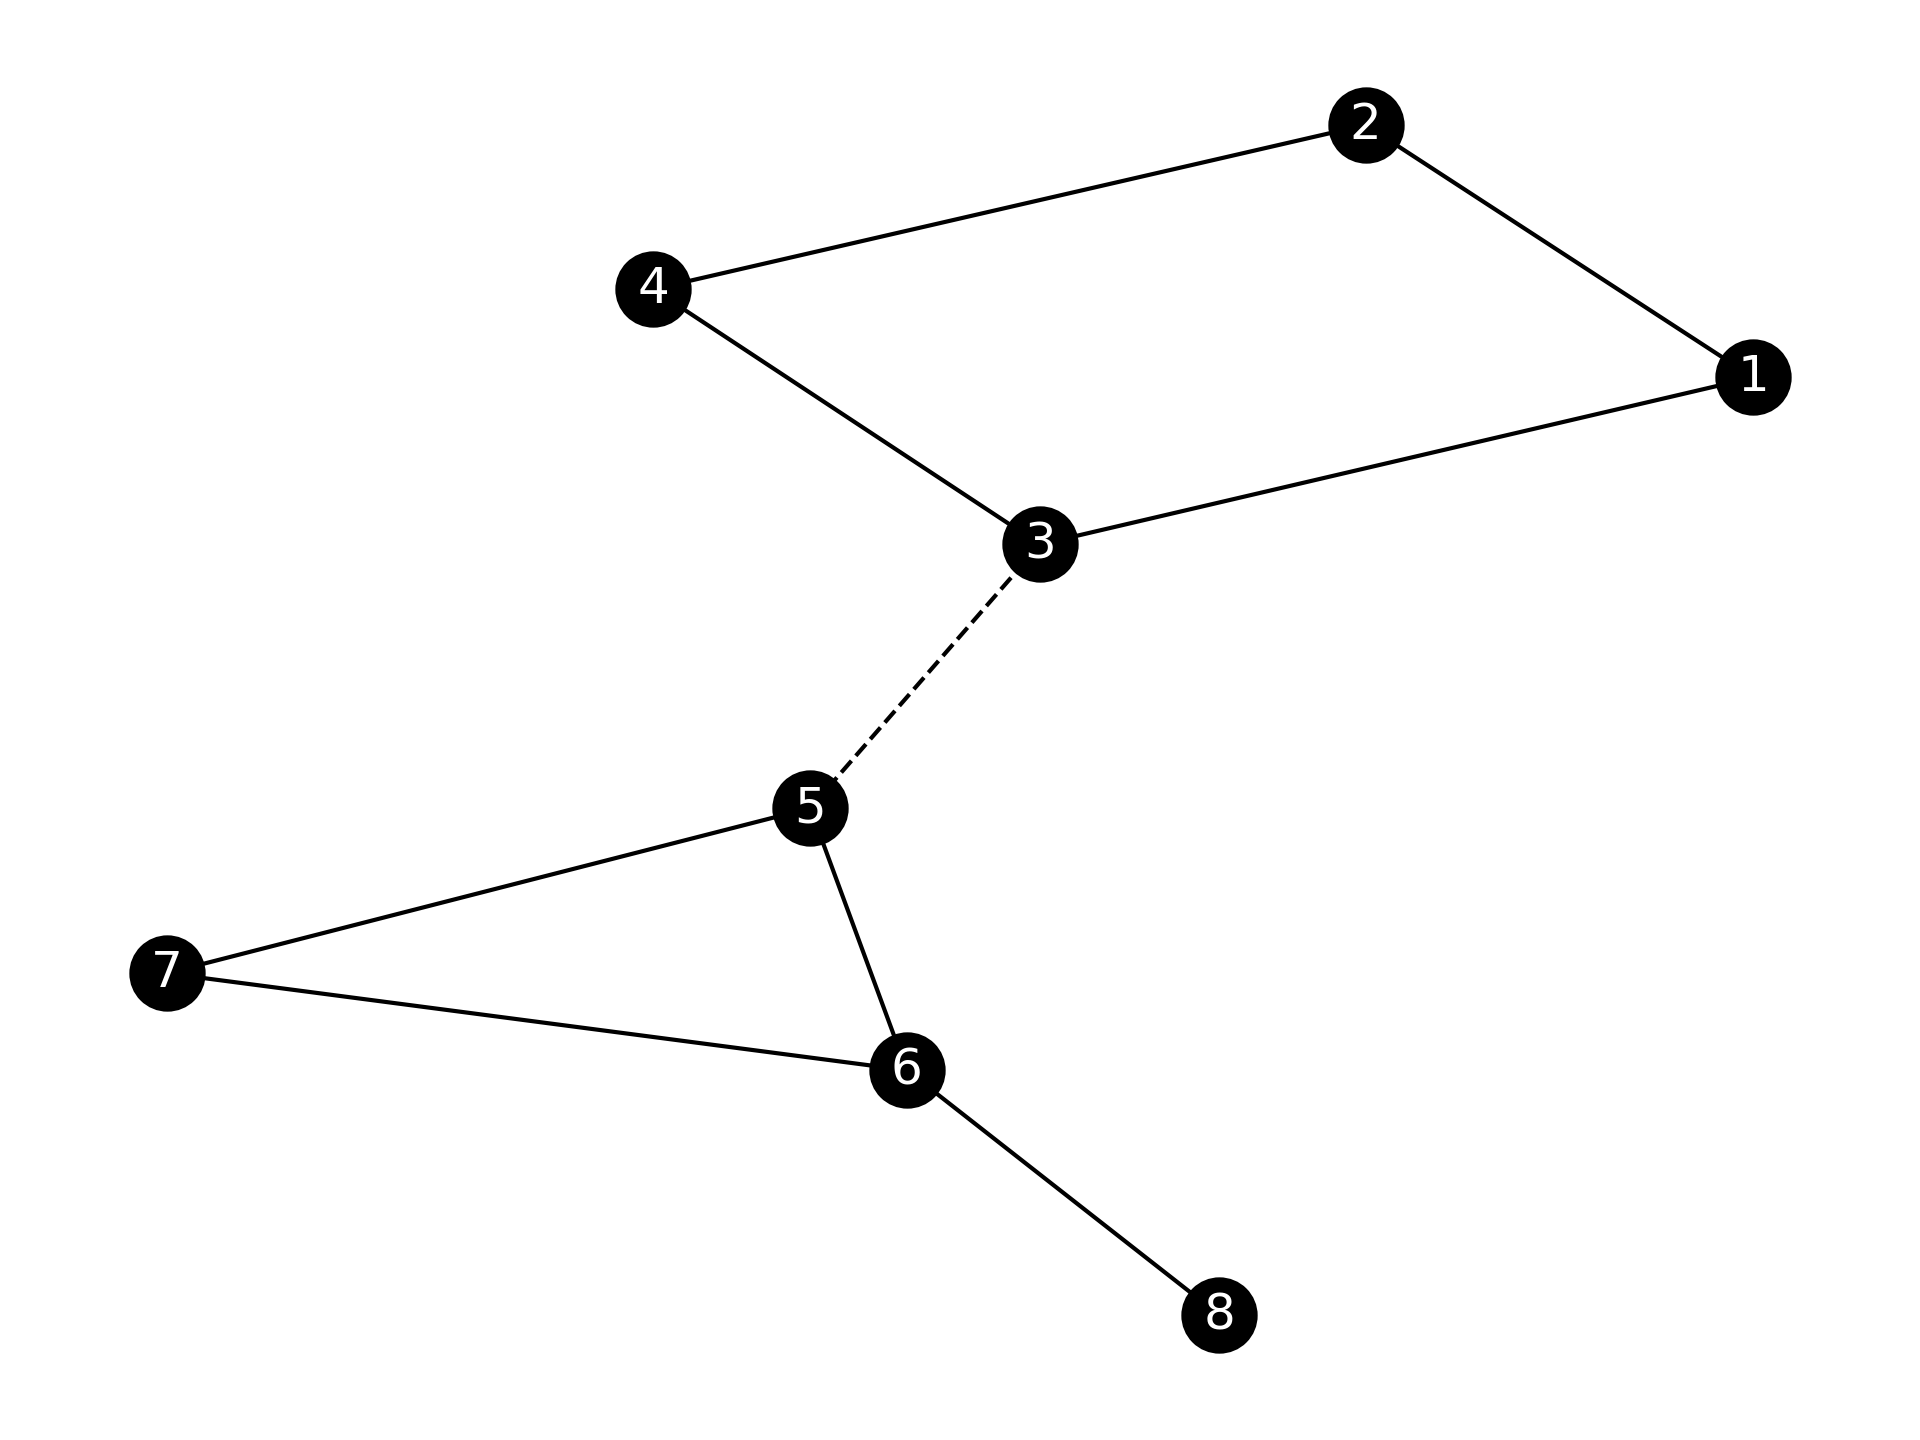
\includegraphics[width=.6\linewidth]{img/atomic_island.png}
    \end{center}
    \caption{
        Example grid topology with 8 nodes and 9 edges. Switches
        are drawn as a dashed line
    }
    \label{fig:data_prep:atomic_islands}
\end{figure}

To do this algorithmically the edges are considered in edge list
form (\ref{eq:graph_theory:edge_list}). They can then be iterated over.
The nodes are initially put into their own atomic island by themselves.
For each edge that is not a switch, each of the atomic islands on either
side are merged.

\begin{algorithm}[h!]
    \LinesNumbered
    \SetAlgoNoEnd
    \SetAlgoVlined
    \DontPrintSemicolon

    \SetKwFunction{GetConnectedIslands}{getConnectedIslands} % Define the function name
    \SetKwProg{Fn}{Function}{:}{} % Define the keyword and formatting
    \SetKwFunction{GetRandom}{getRandom}

    \SetKw{New}{new}
    \SetKwFunction{Dict}{Dict}

    \Fn{\GetConnectedIslands{$nodes$, $edges$}}{

        \tcp{Initialize all nodes within their own islands and create node to island lookup}
        $I \gets $ \{\}\;
        $islandOfNode \gets $ \New \Dict{}\;

        \ForEach{$node \in nodes$}{
            $I_i \gets   \{ node \}$\;
            $I \gets I \cup \{I_i$\}\;
            $islandOfNode[i] \gets I_i$\;
        }

        \tcp{For any edges merge the islands of the nodes on either end}
        \ForEach{$(i, j) \in edges$}{

            \tcp{Remove the old islands}
            $I \gets I \setminus {islandOfNode[i]}$\;
            $I \gets I \setminus {islandOfNode[j]}$\;

            \tcp{Make a new merged island, update lookup and add that island to the overall list}
            $M \gets islandOfNode[i] \cup islandOfNode[j]$\;
            \ForEach{$k \in M$}{
                $islandOfNode[i] \gets M$\;
            }

            $I \gets I \cup \{M\}$\;
        }
    
        \KwRet $I$\;
    }

    \caption{
        Algorithm to obtain all connected subgraphs (or islands) within a given graph, by providing
        a set of $nodes$ and a set of $edges$ as defined in \autoref{eq:graph_theory:edge_list}
    }
    \label{alg:data_prep:atomic_islands}
\end{algorithm}

\autoref{alg:data_prep:atomic_islands} yields the atomic islands if invoked 
with switches removed from the list of edges:

\begin{equation}
    input = edges \setminus switches
\end{equation}

The same algorithm can be used to generate any other kind of connected subgraphs,
depending on the edges removed.\\
\\
Applying \ref{alg:data_prep:atomic_islands} to the grid area mentioned in table \ref{table:data_prep:swiss_suburban_numbers},
produces an atomic island structure depicted in figure \ref{fig:data_prep:swiss_suburb_with_leafs}.

\begin{figure}[H]
    \begin{center}
        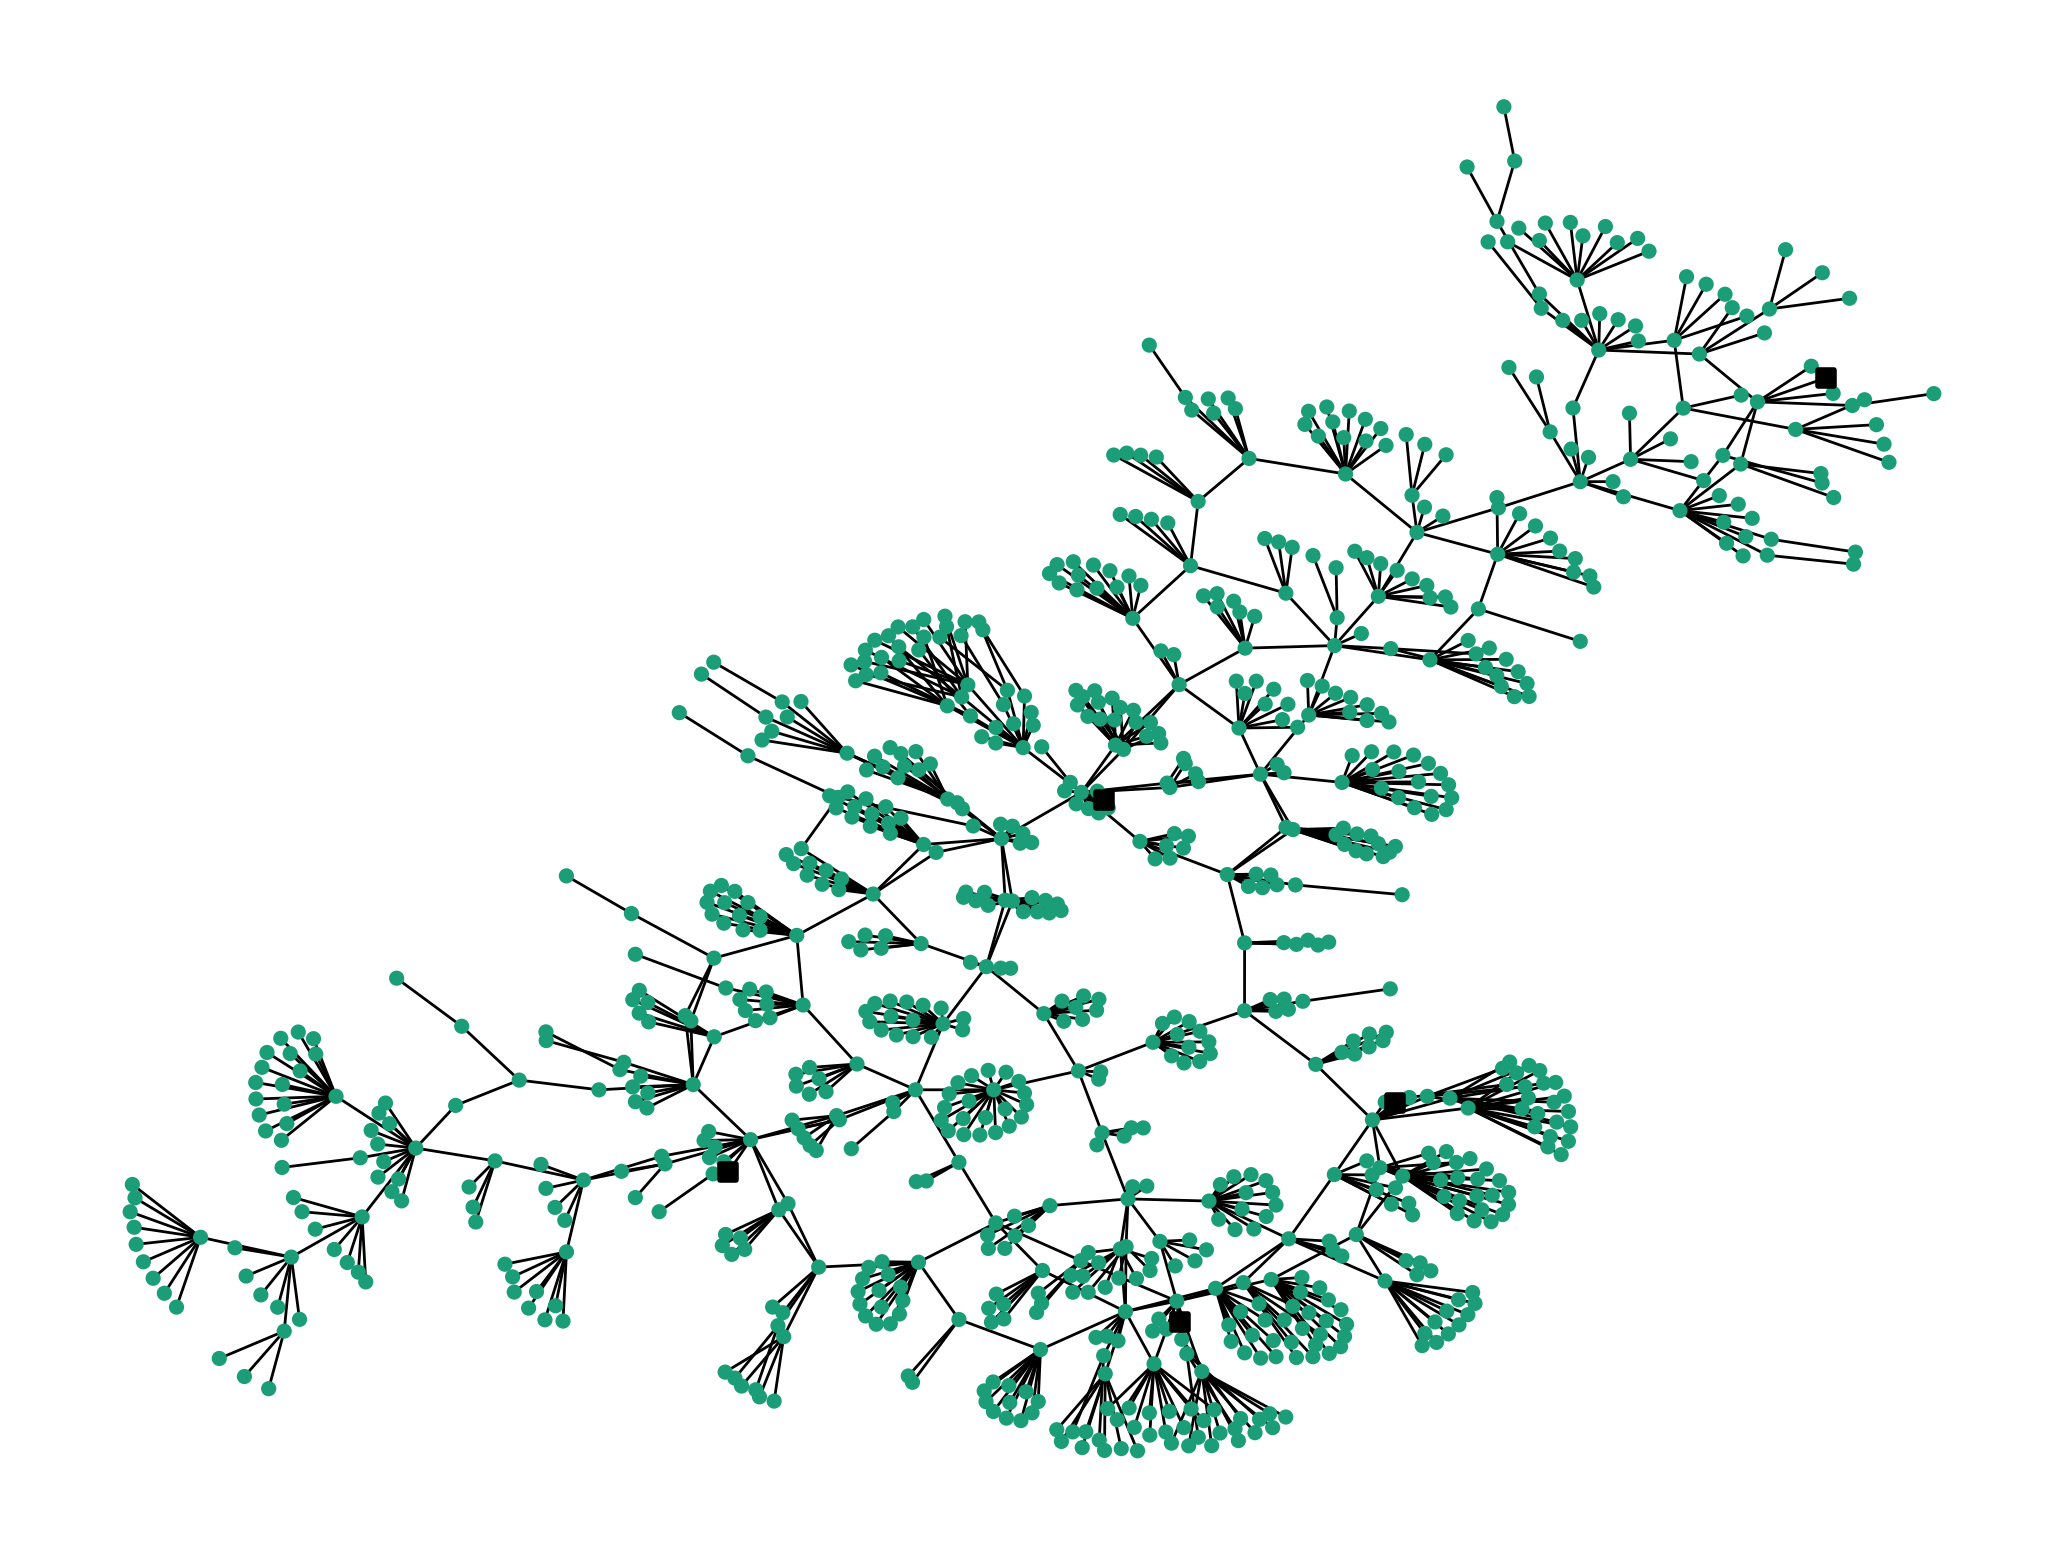
\includegraphics[width=.7\linewidth]{img/switchstate_exploring/swiss_suburb/topology_with_leafs.png}
    \end{center}
    \caption{
        Atomic islands formed out of swiss suburban grid data, laid out in a non-geographical way.
        Atomic islands shown as nodes with 
        ordinary islands in green and islands with transformers as black squares. Connecting switches between the
        atomic islands are shown as edges. Layout produced with
        Kamada-Kawai layout algorithm\autocite{kamada_kawai}.
    }
    \label{fig:data_prep:swiss_suburb_with_leafs}
\end{figure}

From figure \ref{fig:data_prep:swiss_suburb_with_leafs} it can be seen, that
there are a lot of leaf nodes present. A leaf node is a node that only has
one connection in the graph structure. I.e. it is a "dead end" within the graph.
For switch state analysis these nodes are not interesting, as the switch leading
up to them can never be open as that would disconnect that leaf node and thus
disconnect the prosumers in that area.\\
This presents us with an opportunity to
reduce the number of nodes and connections needing to be examined further. Reducing the number of
nodes has considerable benefits later on as it speeds up any algorithm
searching through switch state possibilities. It also makes it visually clearer
what the switchable structure of the grid looks like. \\
We can get rid of the leaf nodes by merging them into their neighbouring nodes. 
After merging a leaf into its neighbour the resulting node might now be a leaf. Thus 
the leaf merging algorithm is repeated until there are no leaf nodes left. In the example
case this reduces the number of atomic islands by 801.

\begin{figure}[H]
    \begin{center}
        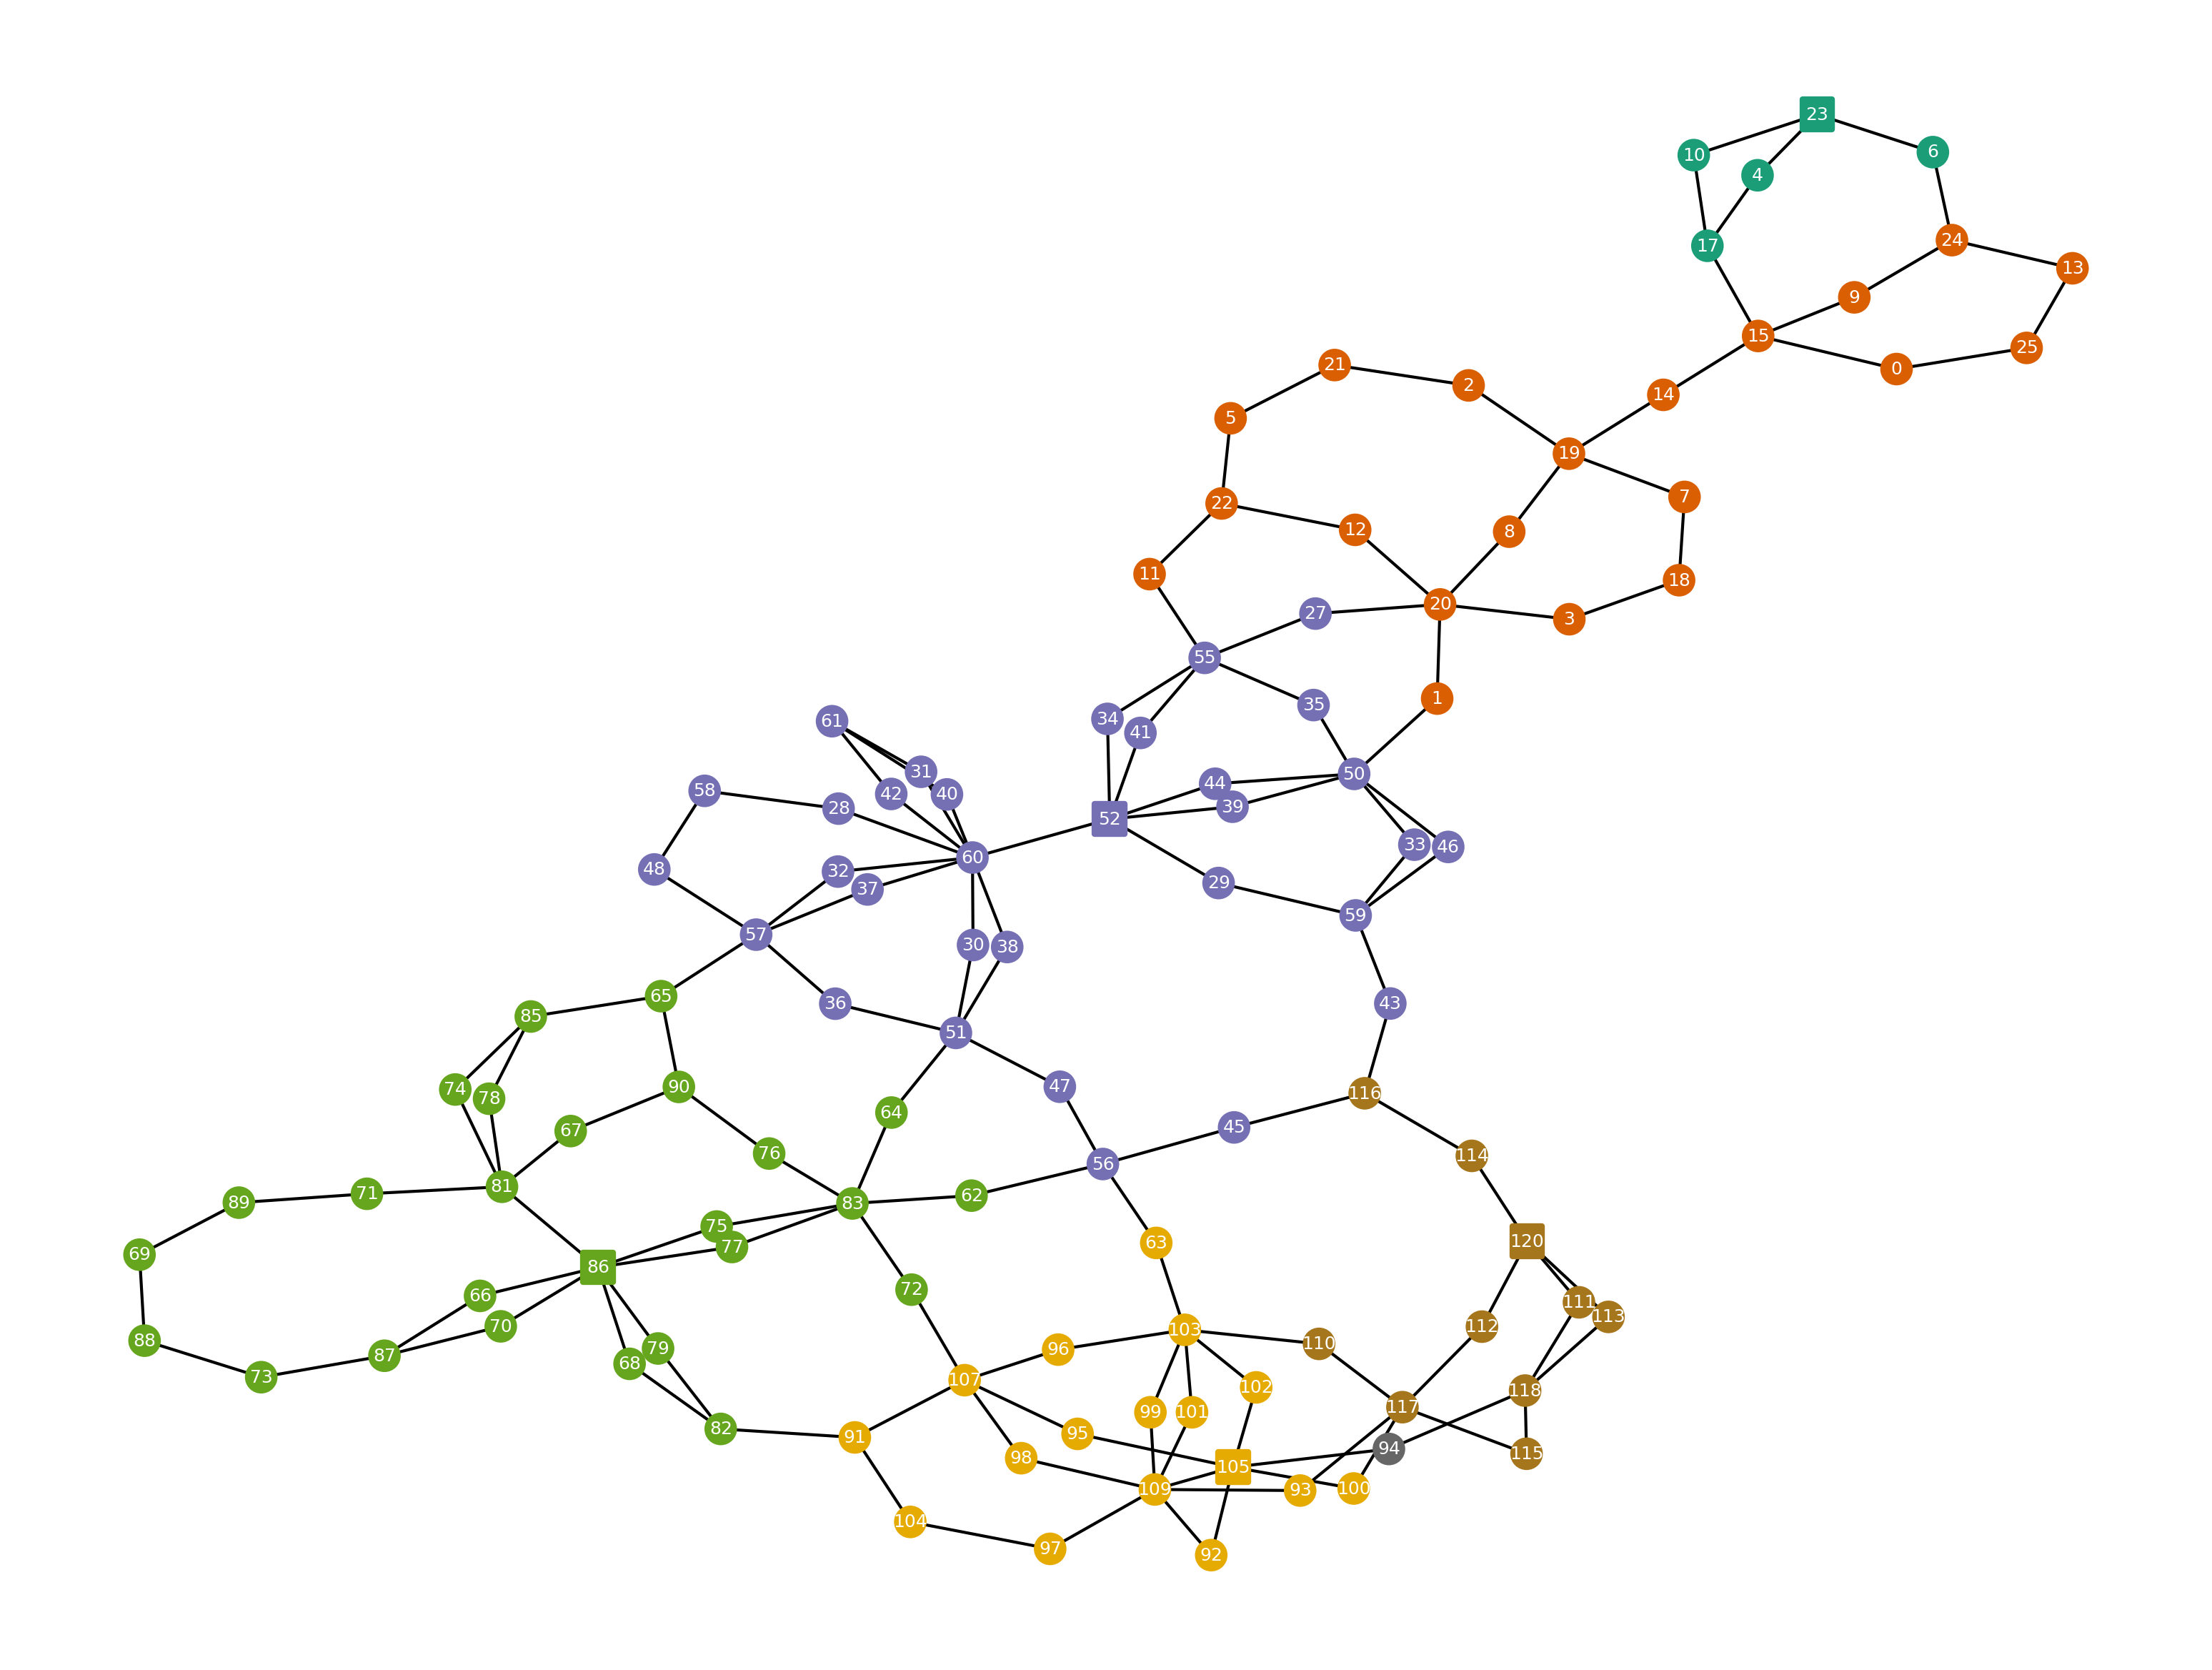
\includegraphics[width=.8\linewidth]{img/switchstate_exploring/swiss_suburb/topology_sss.png}
    \end{center}
    \caption{
        Atomic islands formed out of Swiss suburban grid data, laid out in a non-geographical way.
        Ordinary atomic islands shown as circles, atomic islands with transformer as squares. Atomic islands connected in the
        standard switch case shown as the same colour. Leaf atomic islands merged.
    }
    \label{fig:data_prep:swiss_suburb_topology}
\end{figure}

The last step in data preparation is to determine the standard switch state (SSS). The standard switch
state is the switch state that the grid is in if there are currently no faults or other abnormal
switching being done. I.e. it is the design switch state that the grid operator currently wants the
grid to be in. It is thus also reasonable to later compare any switch state changes to
the SSS and use it as a benchmark. To determine the SSS
an algorithm like algorithm \ref{alg:data_prep:atomic_islands} can be used again, with the nodes being
the atomic islands and the edges being all switches that are closed in the SSS.\\
\\
Lastly can be the case that there end up being atomic islands that are not connected to any
transformer in the SSS. This can happen if there is another neighbouring grid outwith the selected
geographical bounds or due to data quality issues. To rectify this atomic islands like these will
be merged into the island with the least overall grid load. This is to attempt and balance out
the load on the transformer and make the SSS perform the best it can. In the example
there are two clusters of unconnected atomic islands.
Node 94 (grey) and the orange cluster of nodes.
The result of merging them can be seen in \autoref{fig:data_prep:swiss_suburb_topology_patched}.

\begin{figure}[H]
    \begin{center}
        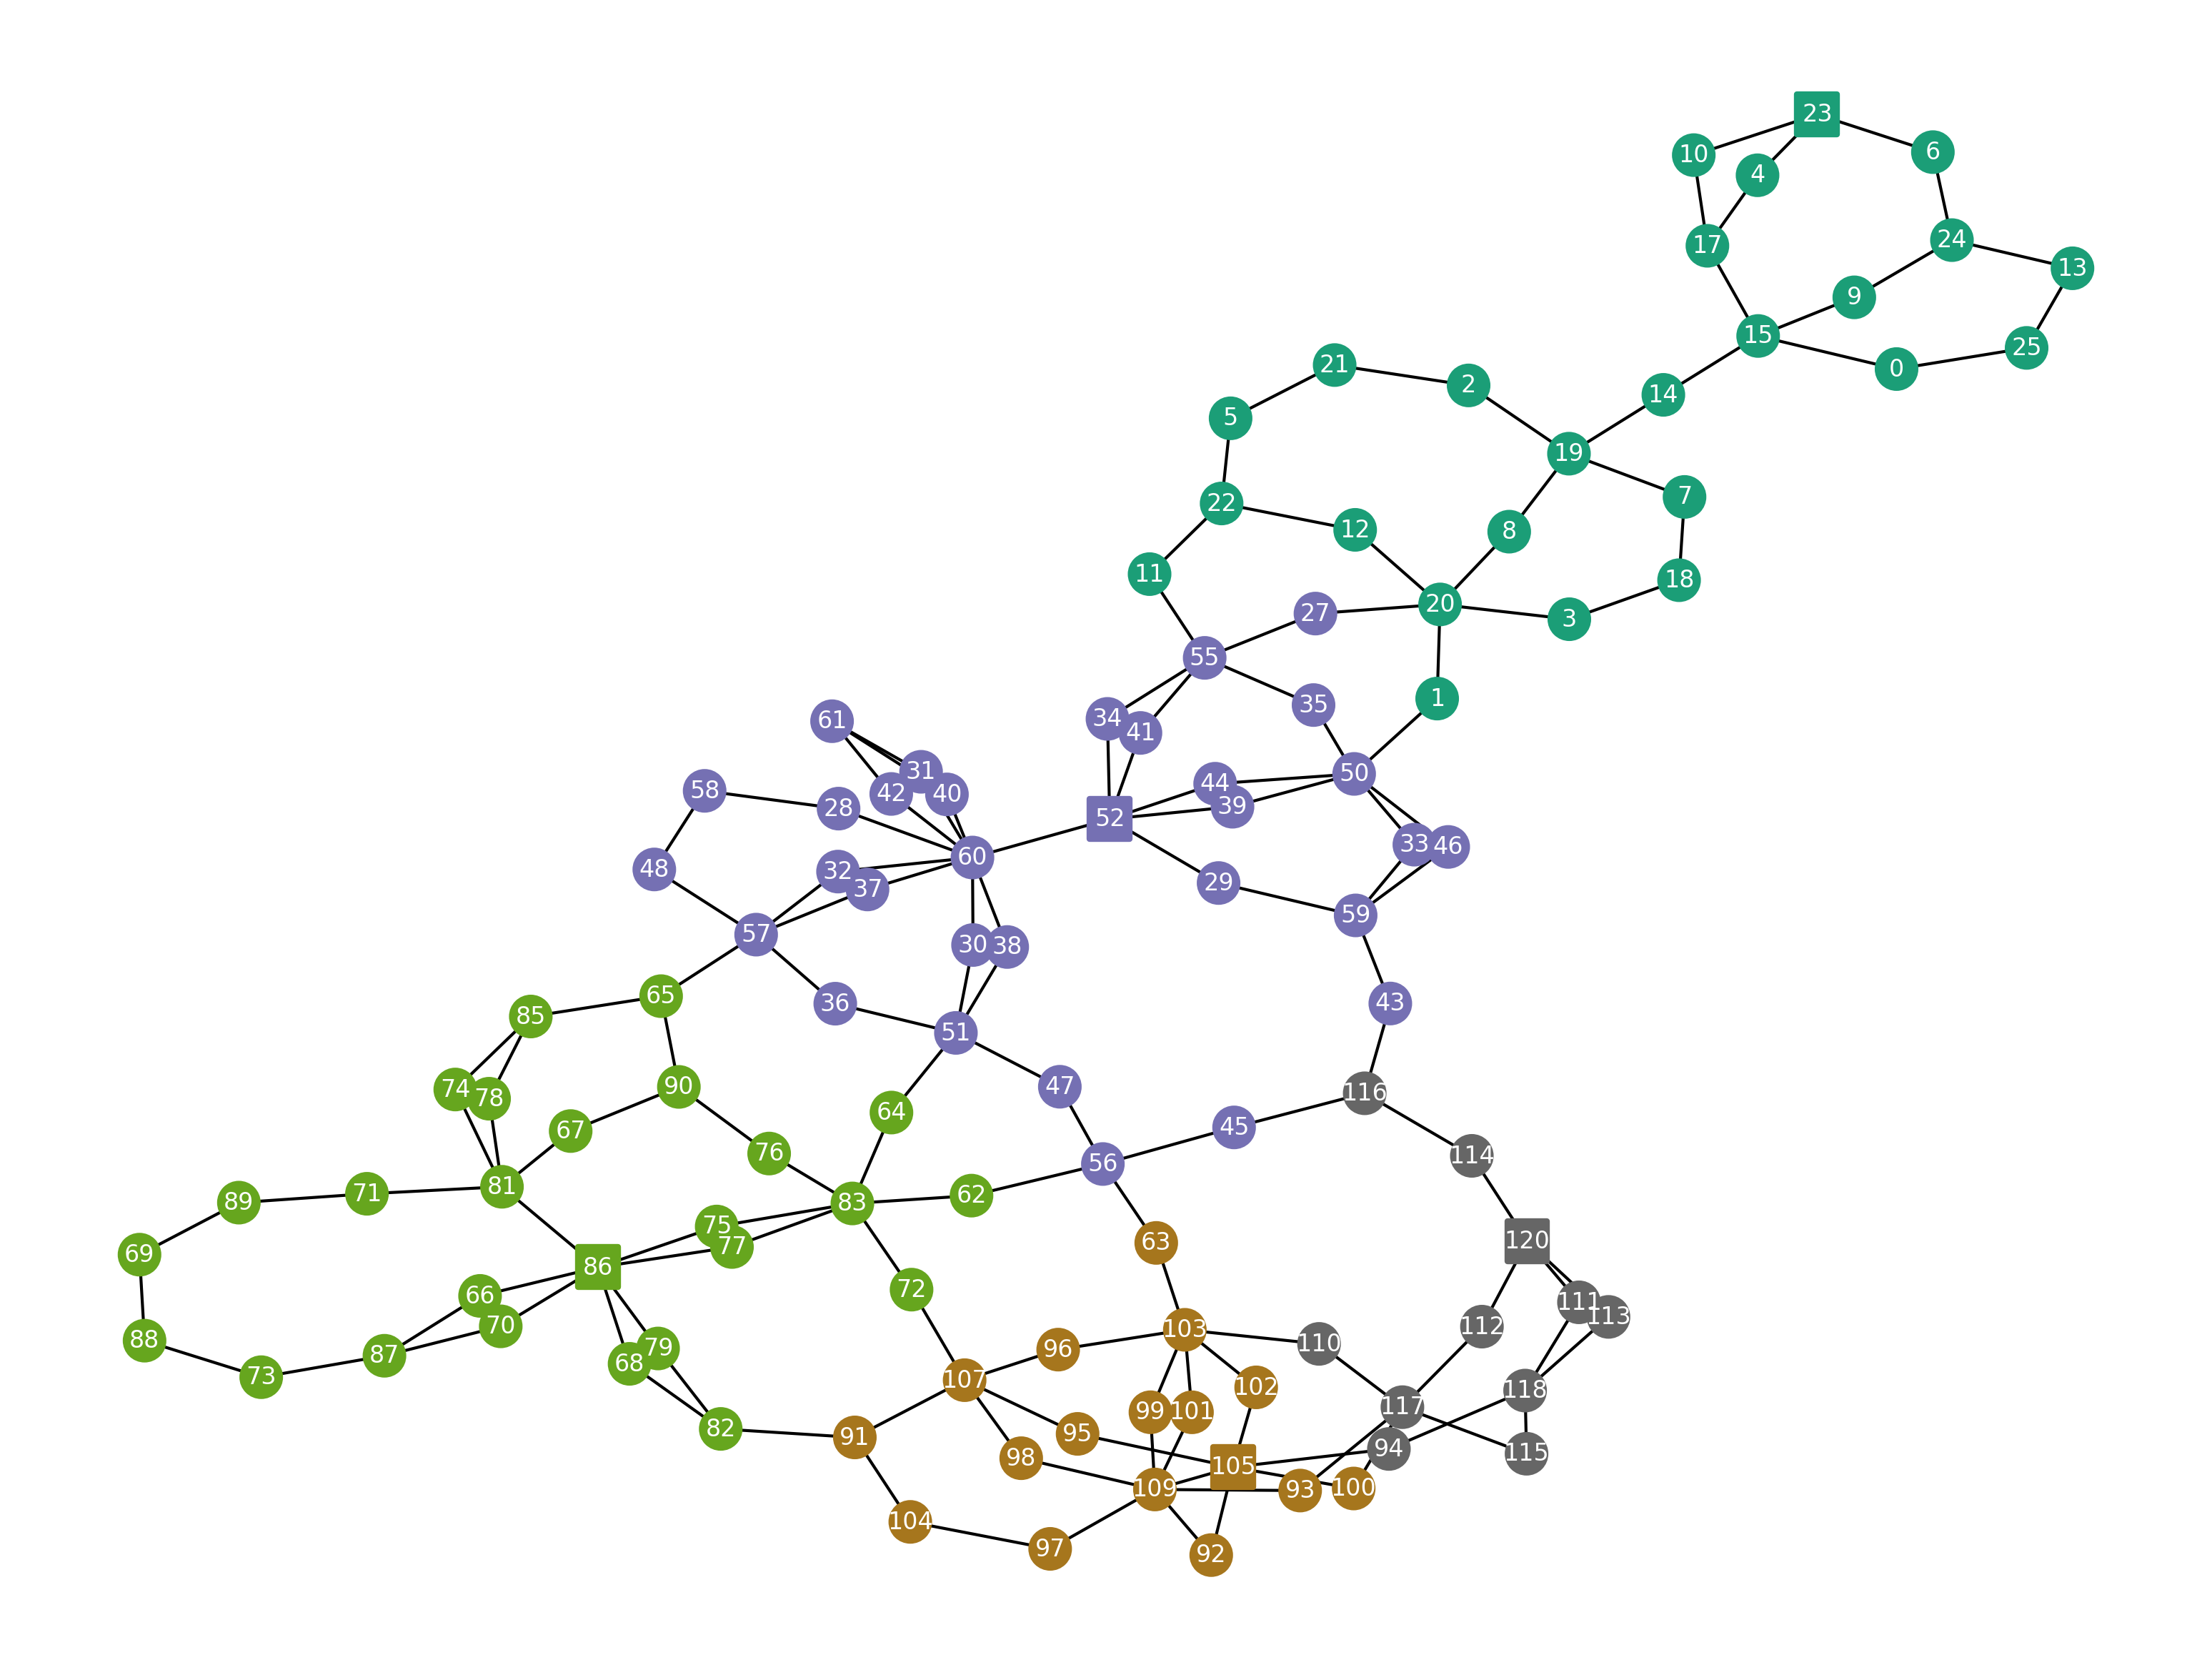
\includegraphics[width=.8\linewidth]{img/switchstate_exploring/swiss_suburb/topology_sss_patched.png}
    \end{center}
    \caption{
        Atomic islands from \autoref{fig:data_prep:swiss_suburb_topology} with unconnected islands
        connected to their neighbour with the lowest net consumption. Layout produced with
        Kamada-Kawai layout algorithm\autocite{kamada_kawai}.
    }
    \label{fig:data_prep:swiss_suburb_topology_patched}
\end{figure}

\subsection{Preparing the data for power flow}

A switch state, defined as a set of templates, provides information
on which atomic islands should be in one power flow island together.
One atomic island however contains many edges and nodes. For power flow
these are the relevant components. Thus, as a first step the set of
all components ending up in a power flow island together have to be formed.
As each atomic island is a set of nodes, the set of nodes in a power flow
island is simply the union of all atomic islands:

\begin{equation}
    \mathfrak{N}_t = \cup_{I \in T_t} I,
\end{equation}

where $\mathfrak{N}_t$ is the set of nodes in template $T_t$
and $I$ an atomic within template $T_t$.\\
\\
All edges within a template ($\mathfrak{E}_t$) 
can be gathered by forming
the subset of edges where both side $i$ and $j$ of
that edge are contained in set of nodes for that template:

\begin{equation}
    \mathfrak{E}_t = \{ \mathfrak{E}_{ij} \in \mathfrak{E} : i, j \in \mathfrak{N}_t \},
\end{equation}

where $\mathfrak{E}$ is the set of all edges as
defined in \autoref{eq:graph_theory:edge_list}.\\
\\
$\mathfrak{E}_t$ contains all edges of all types (see \autoref{table:vep:edges}).
However, the powerflow equation can only be solved for edges
with a non-zero impedance. To solve this we merge all nodes with
zero impedance edges between them into a single node. These nodes
will be called power flow nodes $nodes_{pf}$. To obtain these
\autoref{alg:data_prep:atomic_islands} can be used again. This time
we call it with the subset of edges of zero impedance:

\begin{equation}
    edges_{zero \ impedance} = \{ \mathfrak{E}_{ij} \in \mathfrak{E}_t : Z_{ij} = 0 \}
\end{equation}

and all nodes of the template $\mathfrak{N}_t$. \\
\\

\begin{figure}[h]
    \centering
    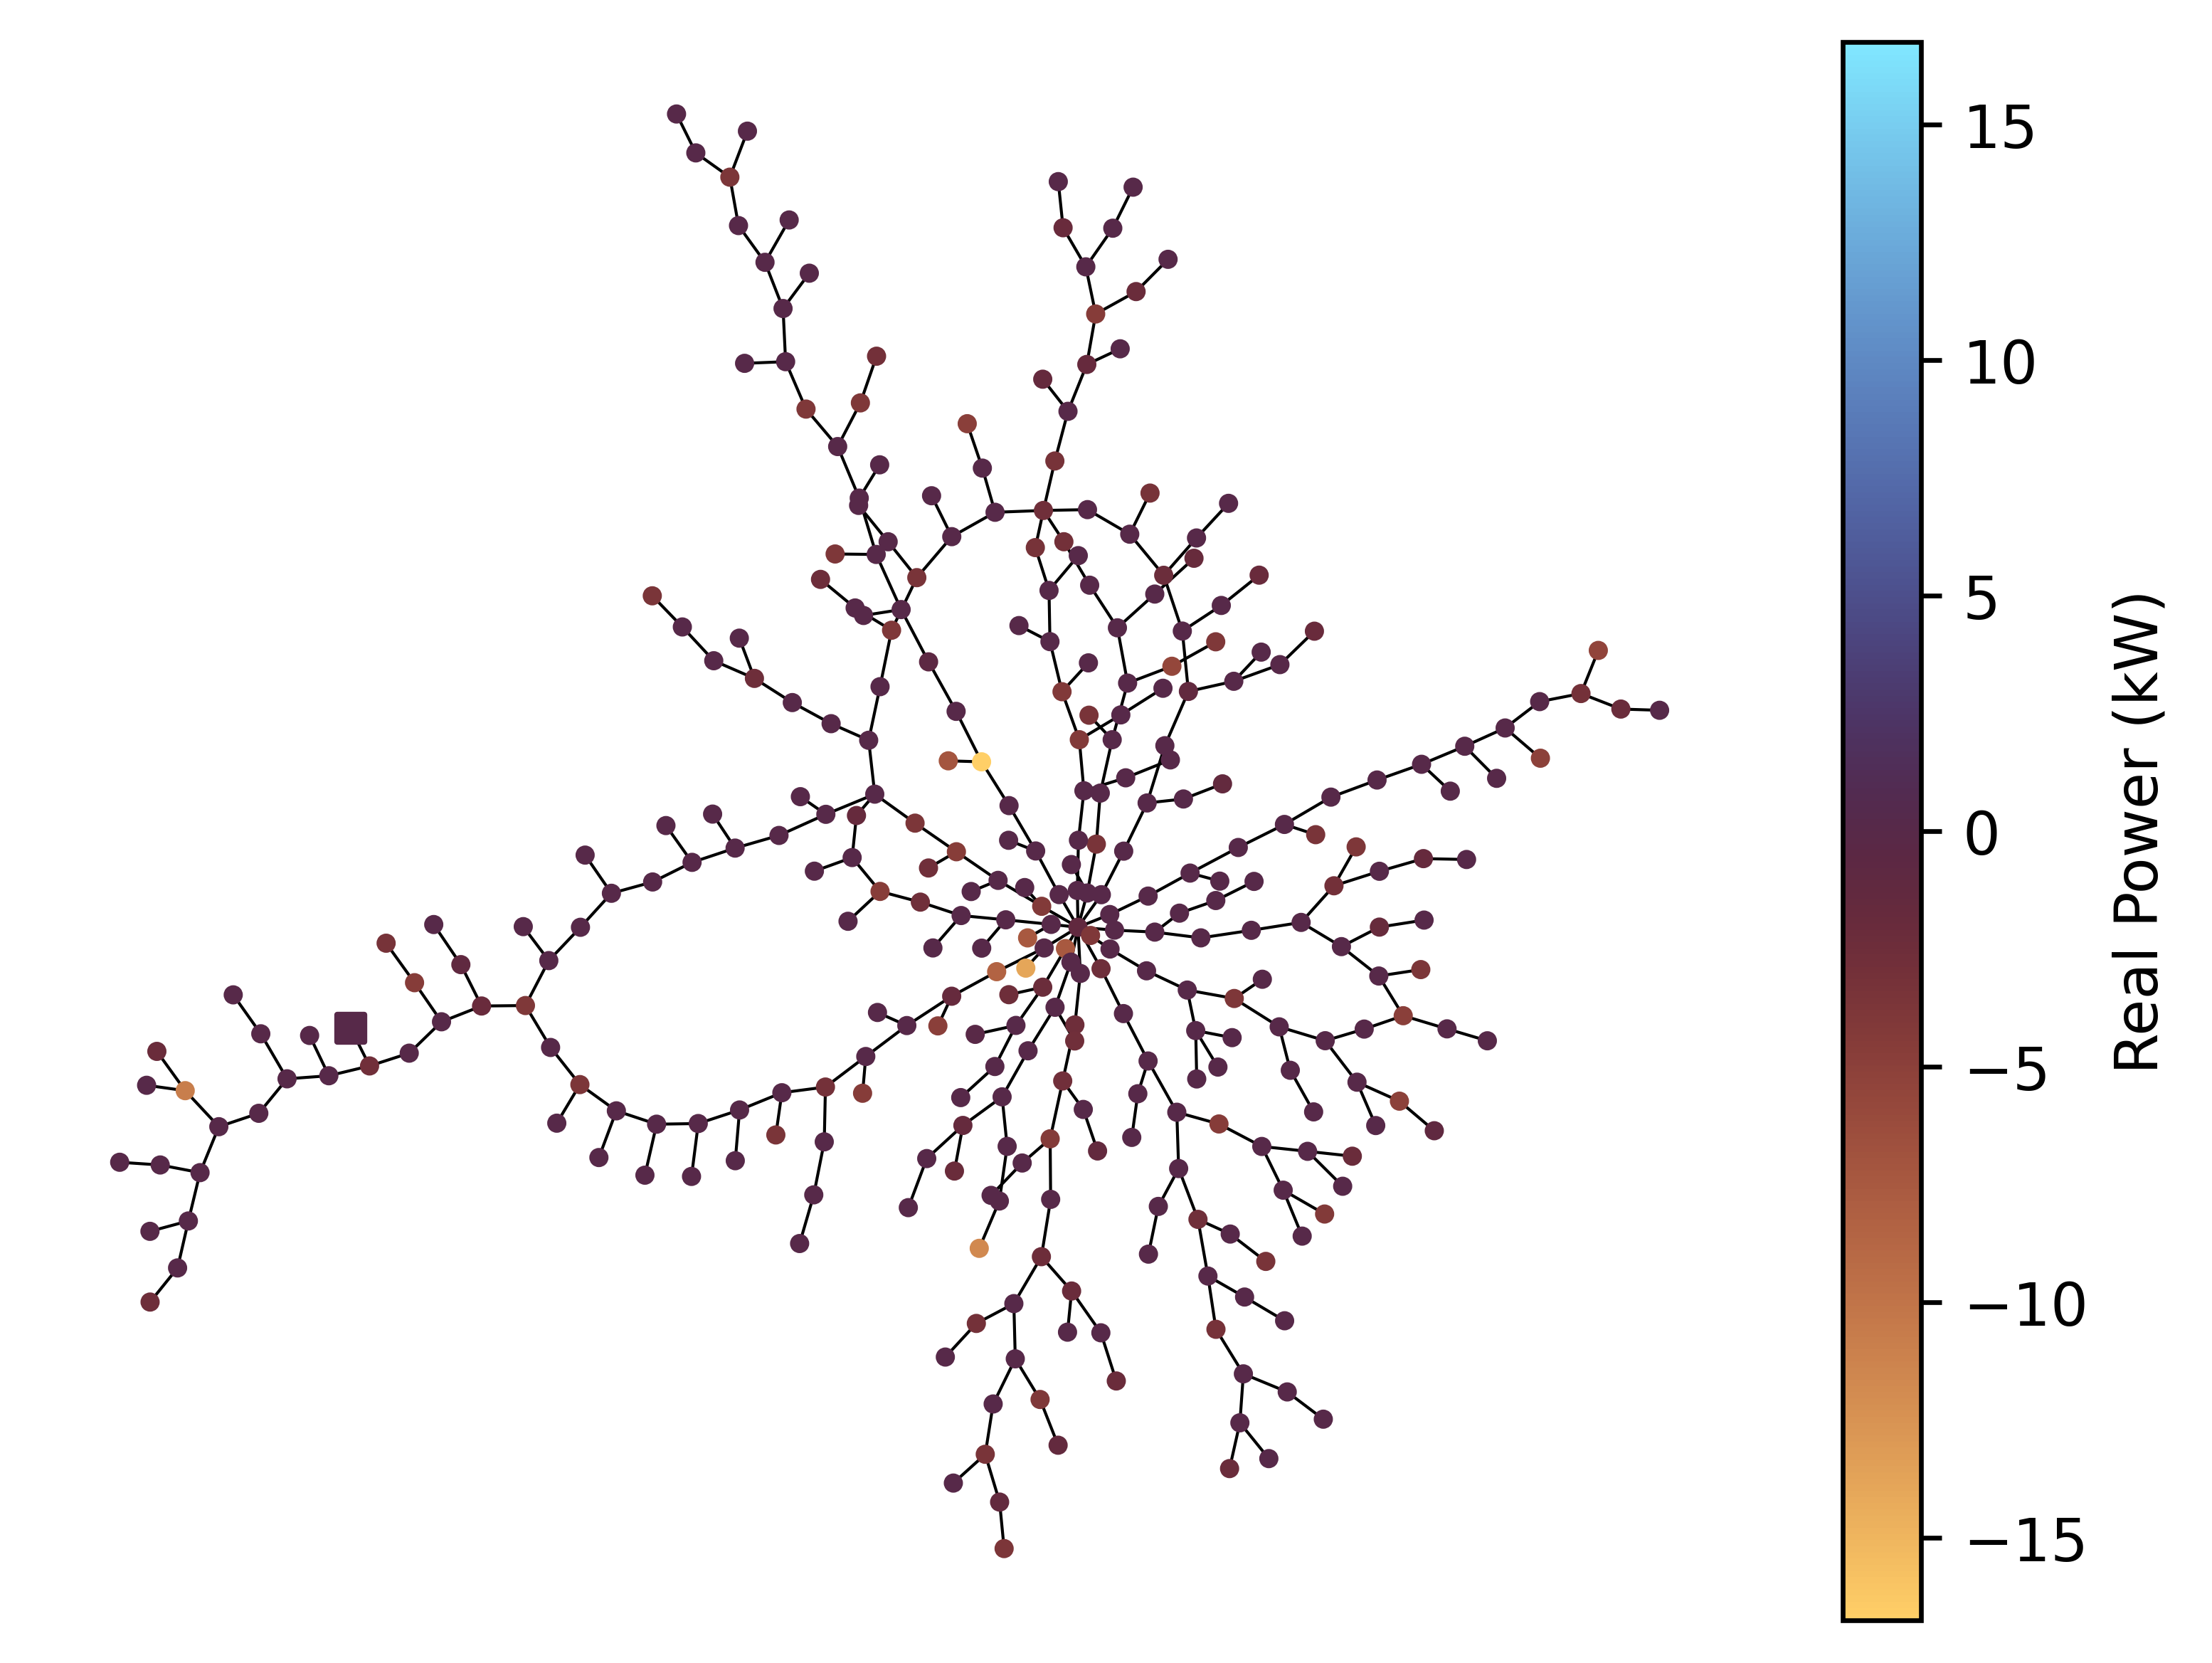
\includegraphics{img/switchstate_exploring/swiss_suburb/pf_island_powers.png}
    \caption{
        Power flow nodes of template 3 (orange) of standard switch state
        of example grid area (see \autoref{fig:data_prep:swiss_suburb_topology_patched}).
        Node coloured by real power $P$. Slack node shown as square. Non-geographical layout using
        Kamada-Kawai algorithm\autocite{kamada_kawai}.
    }
    \label{fig:pf_nodes_power_swiss_suburb}
\end{figure}

For the powerflow algorithm to work we need to designate a slack node. In our
case this will be the power flow node with the transformer connected.
This node is given
index 0 (this becomes important later, see \autoref{sec:pf:impl}). For all
remaining power flow nodes we sum over their constituent nodes to
obtain the total power generated/consumed at that power flow node:

\begin{equation}
    S_i = \sum_{k \in nodes_{pf}} S_k.
\end{equation}

The resulting pf nodes and their real powers $P$ of one of the
templates of the example gird can be
seen in \autoref{fig:pf_nodes_power_swiss_suburb}.\\
\\
All edges with a non-zero impedance are used to form
the admittance matrix $Y$.
As our initial voltage at every node $V_i$ we use the rated
current of the 3-phase low voltage grid $V_{rated} = 400V$.
With this we have all of our constraints to use with
the power flow equations \autoref{eq:pf:gs} or \autoref{eq:pf:nr_pf}.


% Mention how to prepare the data for power flow